
Recall that the goal is to implement the following recurrence :
\begin{align}
\label{eq:convssm_recurrence}
    h_{t+1}=\overline{K}_h{\mathrm{A}} \ast h_t + \overline{K}_x{\mathrm{B}}\ast I_{t+1}
\end{align}
where $h_i$ is the hidden state at time step $i$, $I_i$ is the input image - or feature map. $\overline{K}_h{\mathrm{A}}$ and $\overline{K}_xK_{\mathrm{B}}$ are convolution kernels. For simplicity, we will omit $\overline{K}_xK_{\mathrm{B}}$ in the remainder of this section. We show that computing the sequence of hidden states $(h_i)_{i\in\intint{0}{T-1}}$ given a sequence of inputs $(I_i)_{i\in\intint{0}{T-1}}$ can be seen as computing a scan operation.

We analyse the complexity of the parallel scan algorithm to show why convolutions in spatial domain make the complexity explode, and how doing convolutions in spectral domain preserves $O(\log T)$ complexity. We consider both the work complexity $W$, measuring the total amount of atomic operations to perform, and the time complexity under unlimited parallelization $T_\infty$, measuring the longest sequence of atomic operations remaining after optimal parallelization.

We begin by addressing the main issue of the complexity explosion of convolutional SSMs in \cref{sec:scan_algo,sec:scan_SSM,sec:spatial_ConvSSM,sec:spectral_ConvSSM}. Our main result is \Cref{prop:spectral_conv_complexity}, where we show that we can achieve the same work and time complexity as a regular linear SSM. We then tackle the question of reducing the constant to make it tractable, using standard tricks, adapted to our framework, in \cref{sec:the_constant}.

\paragraph{Mamba-style note.} In this section, we consider transition matrices and transition kernels to be fixed over time. Note that it is entirely possible to have different weights at each time step simply by modifying the initial sequence of $(a_i)_{i\in I}$ defined below. In particular, following \citet{TODO:Mamba} one could parameterize $\Delta$ to depend on the present input $x_i$.

\subsection{The parallel scan algorithm}
\label{sec:scan_algo}

We first describe the parallel scan operation in the most general way. This operation is the core of the SSM parallelization. Let $(a_i)_{i\in I}\in M^I$ be elements of a monoid $(M,+,0)$, with $I=\intint{0}{T\!-\!1}$. The parallel scan is an algorithm that computes $(s_i=\sum_{j=0}^ia_j)_i\in I$. This algorithm is parallelisable and requires associativity of the $+$ operator and a neutral element $0$, hence the minimal requirement of a monoid structure. It proceeds in two sweeps mirroring each other. The first sweep proceeds in a tree like structure, with level $l$ of the tree computing $a^{l+1}_{k}\coloneqq a^l_{2k} + a^l_{2k+1}$, and initialised with $a^0_k\coloneqq a_k$. Once this upward sweep is over, the downward sweep computes mirror operations, with $b^0_1\coloneqq 0$ and $(b^{l+1}_{2k}, b^{l+1}_{2k+1}) = (b^{l}_{k}, b^{l}_{k} + a^{\log_2(T)-(l+1)}_{2k})$. The order is crucial here as $+$ is not required to be commutative. It is only required to be associative. In our application for SSM, it will not be commutative. We denote the parallel scan procedure as $\mathrm{Scan}((a_i)_{i\in I})$ or $\mathrm{Scan}$ for short.
\Cref{fig:parallel_scan_general} provides a visualisation of the entire procedure.

\begin{figure}[ht]
    \centering
    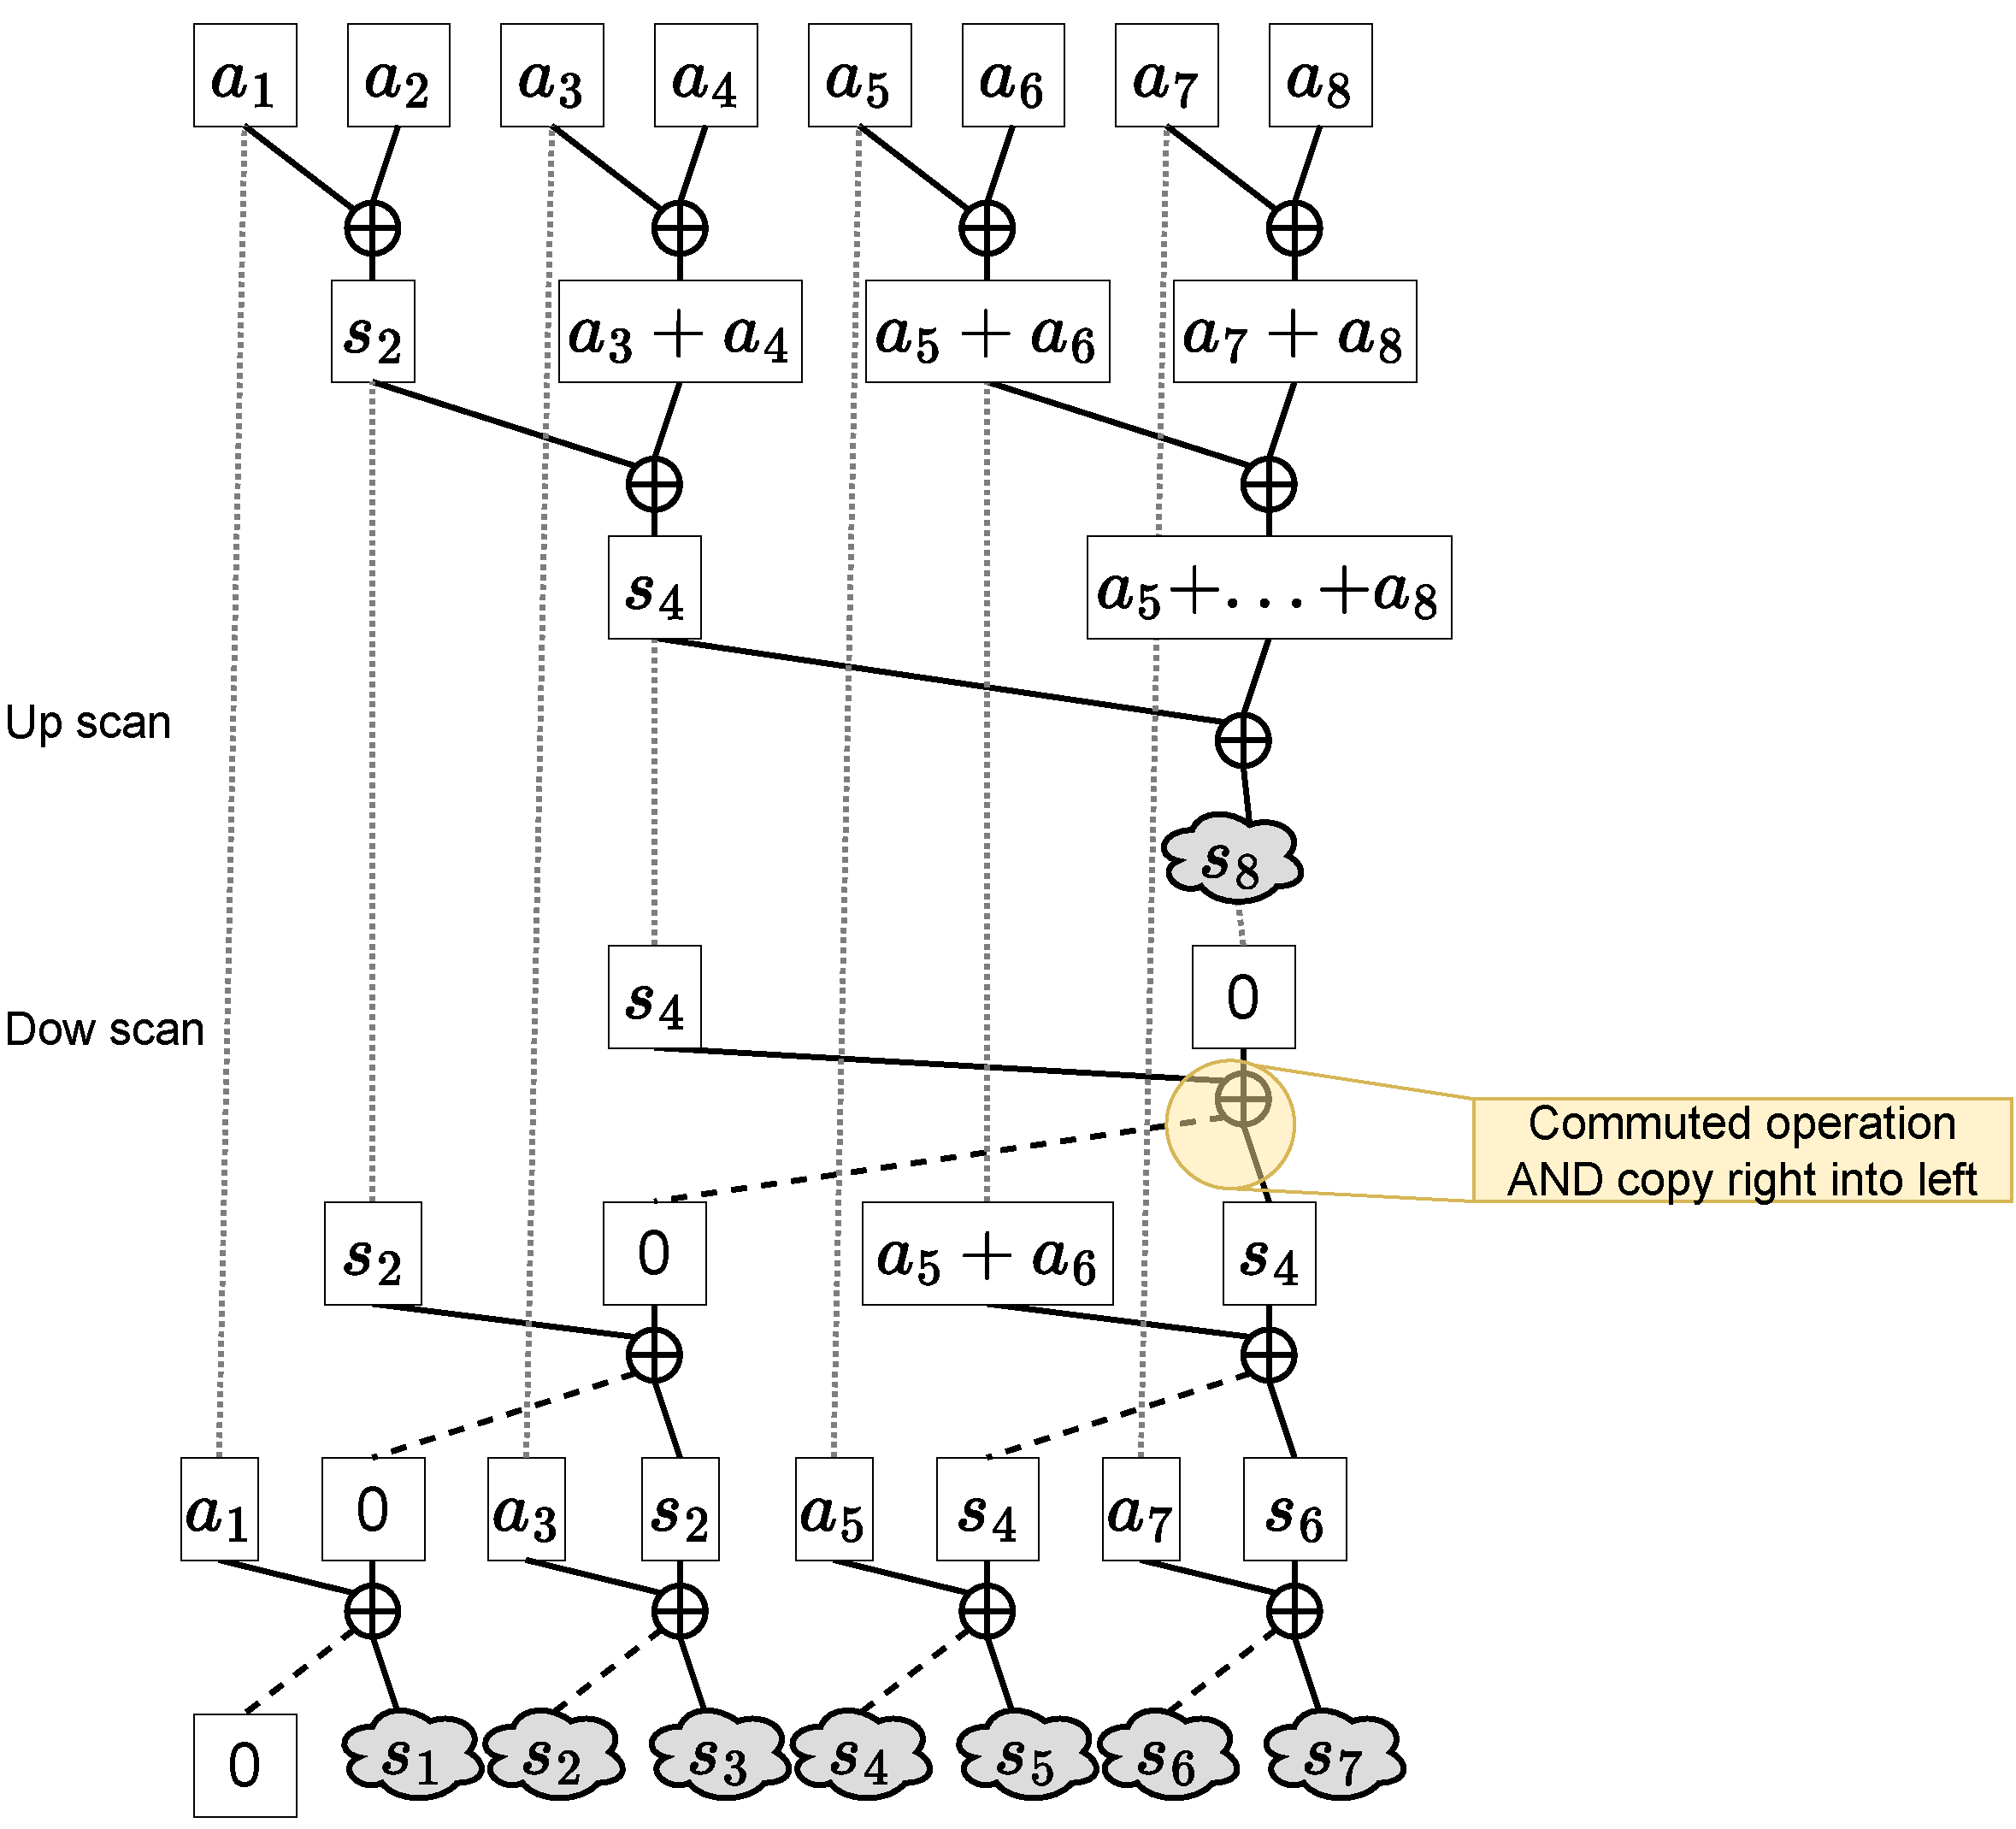
\includegraphics[height=0.3\textheight]{figures/scan_monoid.pdf}
    \hspace{20mm}
    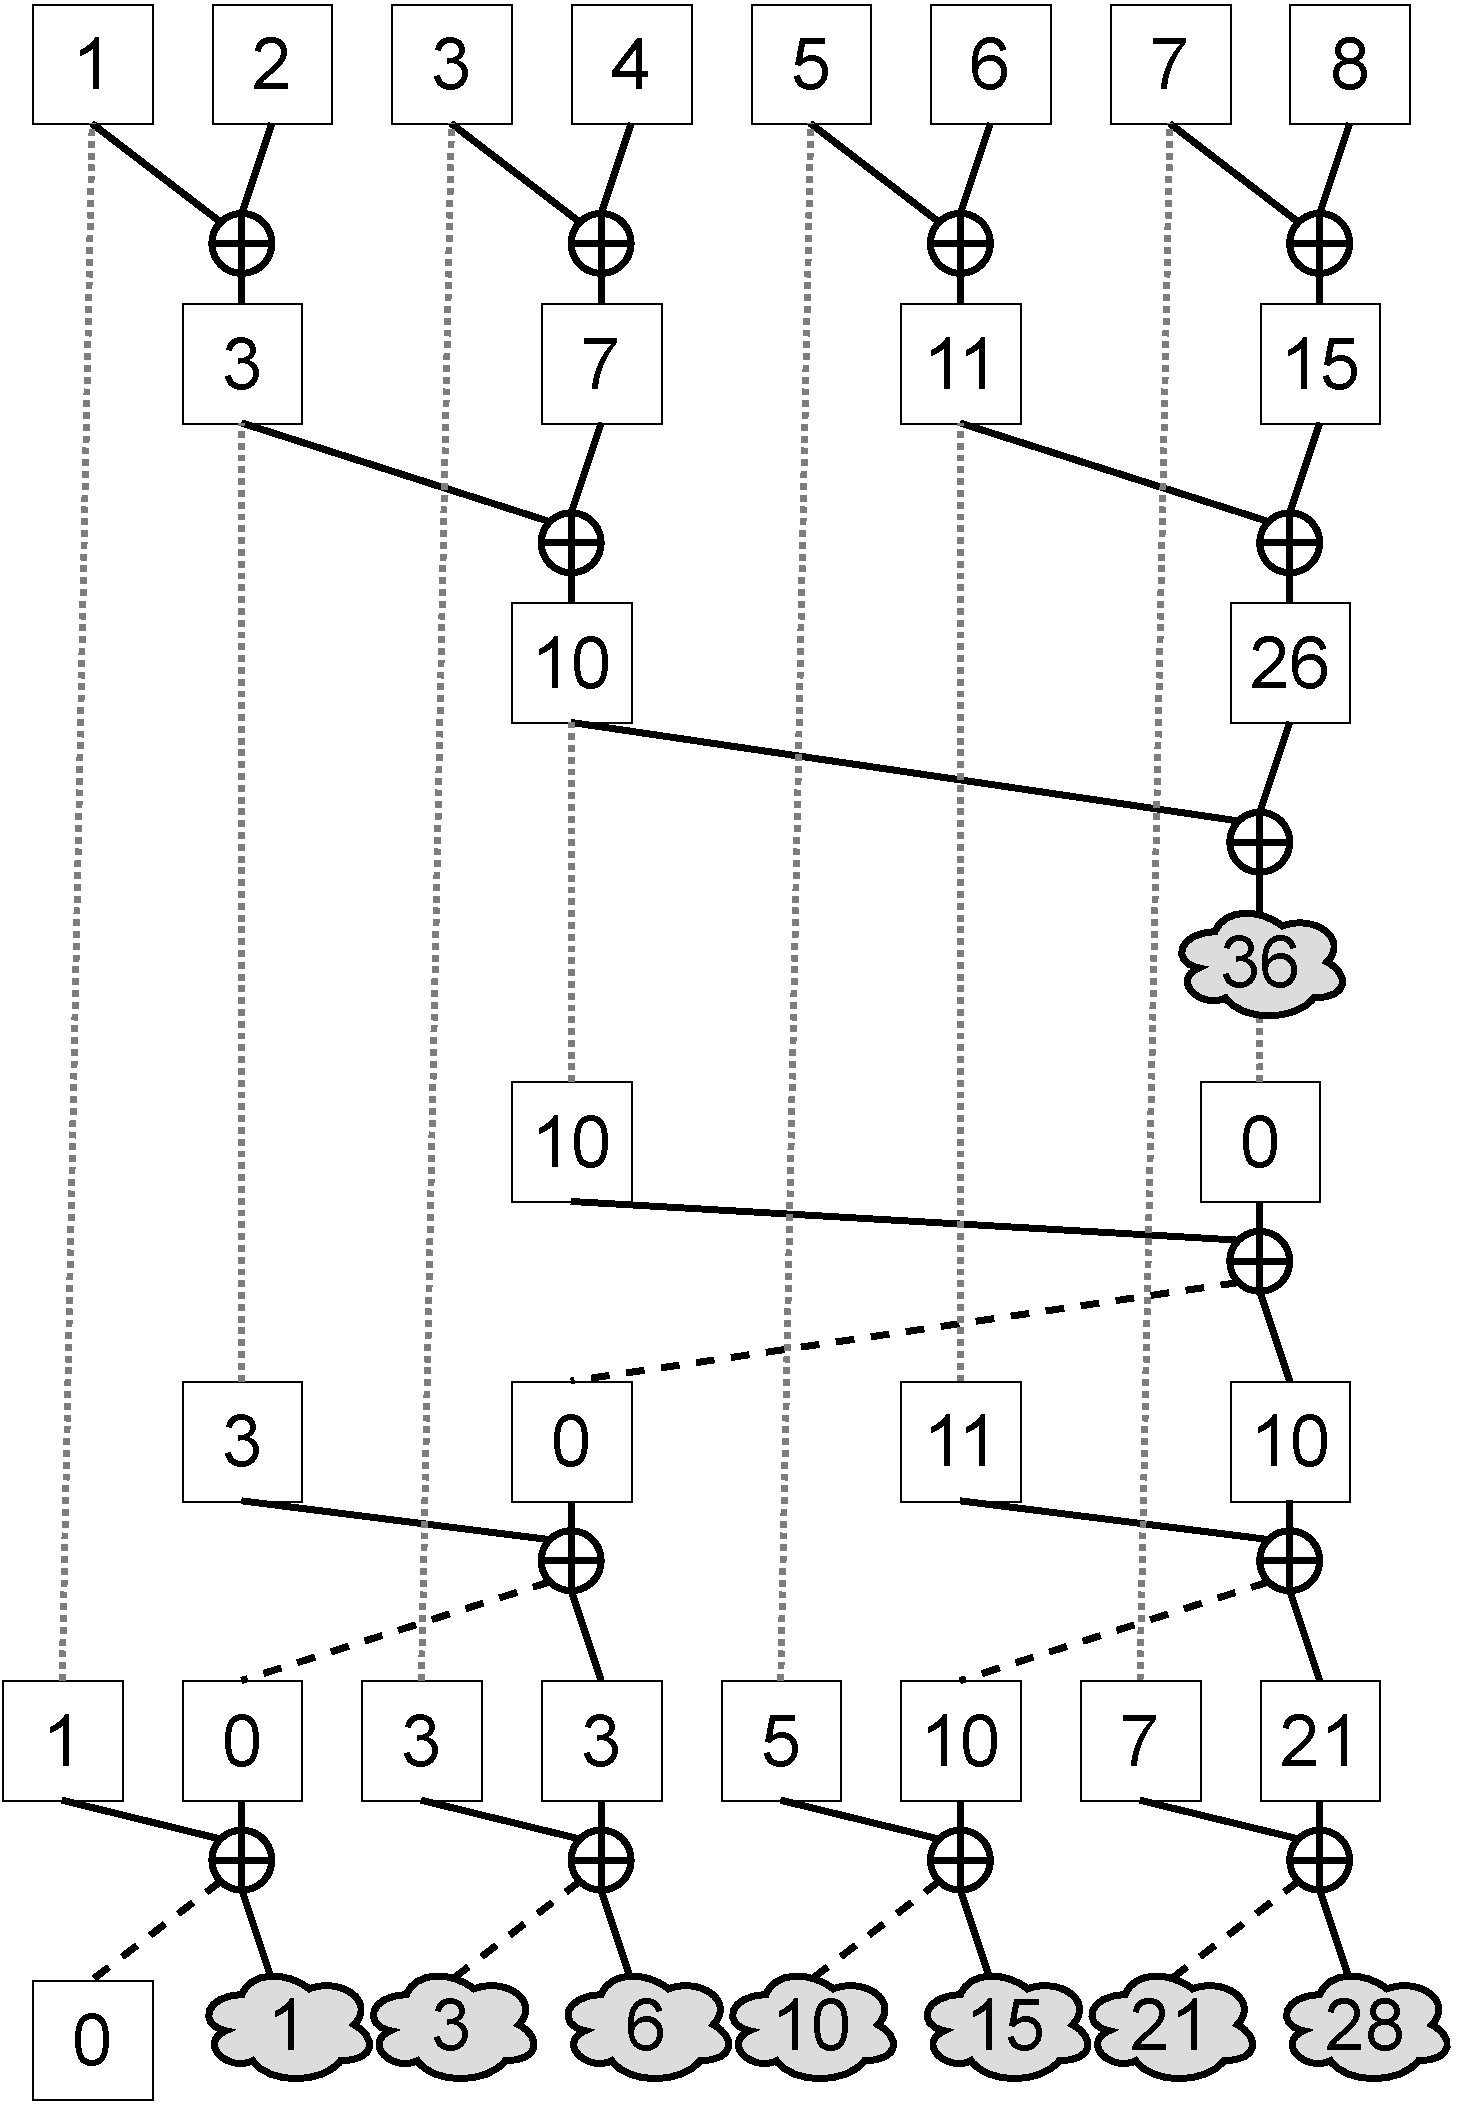
\includegraphics[height=0.3\textheight]{figures/scan_integer.pdf}
    \caption{\textbf{Left:} parallel scan with a generic monoid. \textbf{Right:} illustration on the spetial case of natural integers.}
    \label{fig:parallel_scan_general}
\end{figure}

The procedure described above yields $(\sum_{j=0}^{i-1}a_j)_{i\in I}$, with the cumulative sum being $a^{\log_2(T)}_{0}$ the intermediate result of the upward sweep. We analyse the work complexity $W$ and the time complexity $T_\infty$ of $\mathrm{Scan}$ in terms of floating point operations, where $W$ counts the total number of operations needed and $T_\infty$ counts the time complexity under unlimited parallelism.

\begin{proposition}[Parallel Scan Complexity for $(\N, +)$]
\label{prop:scan_integer_complexity}
    Let $(M, +) \coloneqq (\N, +)$ be the monoid of natural integers equipped with addition. Let $(a_i)_{i\in I}\in \N^I$ be a sequence of integers.

\begin{align}
    W(\mathrm{Scan})&= 2(T-1)\\
    T_\infty(\mathrm{Scan})&= 2\log_2 T
\end{align}
\end{proposition}

\begin{proof}
At level $l$ of the upward scan, $U_l = T/(2^{l+1})$ "$+$" operations are performed, each of them having a complexity of $1$. There are $\log_2 T$ levels in total. The same goes on for the downward scan, with $D_l = T/(2^{\log_2(T) - l})=2^{l}$ operations at level $l$. Therefore, the work complexity of level $l$ is $U_l$ (resp. $D_l$) while its time complexity is $1$ with unlimited parallelism. It follows that

\begin{align}
\label{eq:W_integer}
W &= 2\sum_{l=0}^{\log_2(T)-1}2^l=2(T-1)\\
\label{eq:T_integer}
T_\infty&= 2\sum_{l=0}^{\log_2(T)-1}1=2\log_2T
\end{align}
\end{proof}

\subsection{The case of SSM}
\label{sec:scan_SSM}

The case of SSMs is a little more complicated than that of real numbers. In SSMs, the recurrence is defined by \Cref{eq:convssm_recurrence} with the slight modification that kernel convolution is now matrix multiplication and taking $B = I$. Thus, the goal is to compute in parallel the hidden states $(h_i = \sum_{j=0}^i\overline{A}^{i-j}x_j)_i\in I$, where $x_i$ are vectors of dimension $d$ and $\overline{A}$ is a square matrix. This is almost but not quite what we need for the parallel scan. We define the following monoid:
\begin{align}
\label{eq:M_SSM}
    &M^{\mathrm{SSM}}\coloneqq \left\{a = (A, x)\mid A\!\in\!\mathcal{M}_{d}(\R),~x\!\in\!\R^d\right\}\\
\label{eq:+_SSM}
    &(A_a, x_a) +^{\mathrm{SSM}} (A_b,x_b)\coloneqq (A_b \odot A_a, A_b \cdot x_a + x_b)\\
\label{eq:0_SSM}
    &0^{\mathrm{SSM}}\coloneqq(I_d, 0)
\end{align}

With this monoid structure, and the sequence $(a_i)_{i\in I} \coloneqq ((A, x_i))_{i\in I} \in M^I$, the result of the parallel scan is $((A^i, \sum_{j=0}^iA^{i-j}x_j))_{i\in I}$. The complexity of the scan is less straightforward, but the complexity of each $+^{\mathrm{SSM}}$ operation depends only on $d$, it is a constant of $T$, and therefore, the overall time complexity of the scan is $T_\infty= O(\log T)$ and $W=O(T)$.

\begin{proposition}[SSM Complexity]
\label{prop:SSM_complexity}
    Let $(M, +) \coloneqq (M^{\mathrm{SSM}}, +^{\mathrm{SSM}})$ be the monoid defined by \Cref{eq:M_SSM,eq:+_SSM,eq:0_SSM}. Let $(a_i)_{i\in I}\in (M^{\mathrm{SSM}})^I$.

\begin{align}
    W(\mathrm{Scan})&= 2(T-1)(d^3+d^2+d)\\
    T_\infty(\mathrm{Scan})&= 2\log_2 (T) (d^3+d^2+d)
\end{align}
\end{proposition}

\begin{proof}
The proof of \Cref{prop:scan_integer_complexity} applies with the only difference that now, each $+^{\mathrm{SSM}}$ operation has complexity $d^3$ for the matrix multiplication on the left, $d^2$ for the matrix-vector multiplication and $d$ for the vector addition on the right.
\end{proof}

\subsection{The problem of convolution}
\label{sec:spatial_ConvSSM}

Moving from $d$ dimensional vectors to images with $c$ channels and $h \times w$ spatial dimension and from matrix multiplication to spatial convolution, we can rewrite our monoid structure as :
\begin{align}
    &M^{\mathrm{Conv}_1}\coloneqq \left\{a = (K, I)\mid \exists k_1, k_2,\quad K\!\in\!\R^{k_1\times k_2\times c\times c},~I\!\in\!\R^{h \times w \times c}\right\}\\
    &(K_a, I_a) +^{\mathrm{Conv}_1} (K_b,I_b)\coloneqq (K_b \circledast K_a, K_b \ast I_a + I_b)\\
    &0\coloneqq(I, 0)
\end{align}
\noindent where $\circledast$ is the convolution between two kernels and $\ast$ is the convolution between a kernel and an image:

\begin{align*}
    & \forall \left\{
\begin{aligned}
    &x\!\in\!\intint{0}{h\!-\!1}\\
    &y\!\in\!\intint{0}{w\!-\!1}\\
    &c_{\mathrm{out}}\!\in\!\intint{1}{c}
\end{aligned}
\right., (K\!\ast\!I)_{x,y,c_{\mathrm{out}}} = \sum_{u=0}^{k_1-1}\sum_{v=0}^{k_2-1}\sum_{i=1}^{c} K_{u,v,i,c_{\mathrm{out}}} I_{(x-u,y-v)\%(h,w),i}\\
    & \forall \left\{
\begin{aligned}
    &u\!\in\!\intint{0}{k_1\!+\!l_1\!-\!2}\\
    &v\!\in\!\intint{0}{k_2\!+\!l_2\!-\!2}\\
    &c_{\mathrm{in}},c_{\mathrm{out}}\!\in\!\intint{1}{c}
\end{aligned}
\right., (L \circledast K)_{u,v,c_{\mathrm{in}},c_{\mathrm{out}}} = \sum_{p=0}^{l_1-1}\sum_{q=0}^{l_2-1}\sum_{c_{k}=1}^{c} L_{p,q,c_{k},c_{\mathrm{out}}} K_{u-p,v-q,c_{\mathrm{in}},c_{k}}\text{, $K$ being zero-padded}
\end{align*}
\noindent with $L\!\in\!\R^{l_1\times l_2\times c \times c}$, $K\!\in\!\R^{k_1\times k_2\times c \times c}$ and $I\!\in\!\R^{h \times w \times c}$

With this structure, the key aspect is that the spatial size of the kernel resulting from $\circledast$ is the sum of the sizes of the input kernels. Therefore, the parallel scan algorithm operates on larger and larger kernel sizes, with sizes growing exponentially with the depth in the tree structure. The complexity of our $+$ operator is thus no more constant as it depends on the depth. The bottleneck is at the very last layer of the upward scan, where kernel size is $O(Tk)$, with $k$ the size of the original kernel $K$, resulting in a single $\ast$ operation whose complexity is in $O(T^2)$. This bottleneck is illustrated in \Cref{fig:parallel_scan_conv_spatial}.

\begin{proposition}[Spatial ConvSSM Complexity]
    Let $(M, +) \coloneqq (M^{\mathrm{Conv}_1}, +^{\mathrm{Conv}_1})$ be the monoid defined by \Cref{eq:M_SSM,eq:+_SSM,eq:0_SSM}. Let $(a_i)_{i\in I}\in (M^{\mathrm{Conv}_1})^I$.

\begin{align}
    W&= O(T^2)\\
    T_\infty&= O(W)
\end{align}
\end{proposition}

\begin{proof}
The proof of \Cref{prop:scan_integer_complexity} applies with the major difference that on the upward scan, at level $l$, each $+^{\mathrm{Conv}_1}$ operation has complexity $(k+(2^l-1)(k-1))\times (k+(2^l-1)(k-1))\times c^3 = O((2^l)^2\times k^2 \times c^3)$ for the kernel-kernel convolution on the left, $O(h \times w \times (2^l)^2\times k^2 \times c^2)$ for the kernel-image convolution and $h \times w\times c$ for the image addition on the right. The same goes on for the downward scan.

Thus, \Cref{eq:W_integer,eq:T_integer} become :

\begin{align}
\label{eq:W_conv}
W &= O(2 \sum_{l=0}^{\log_2(T)-1} 2^{\log_2(T)-(l+1)} \times \left[ (2^l)^2\times k^2 \times c^3 + h \times w \times (2^l)^2\times k^2 \times c^2\right])\\
&= O(T^2 \times k^2 \times c^3) + O(T^2 \times h \times w \times k^2 \times c^2)\\
\label{eq:T_conv}
T_\infty&= O(2\sum_{l=0}^{\log_2(T)-1} \left[ (2^l)^2\times k^2 \times c^3 + h \times w \times (2^l)^2\times k^2 \times c^2\right])\\
&= O(W)
\end{align}
\end{proof}

\begin{figure}[ht]
    \centering
    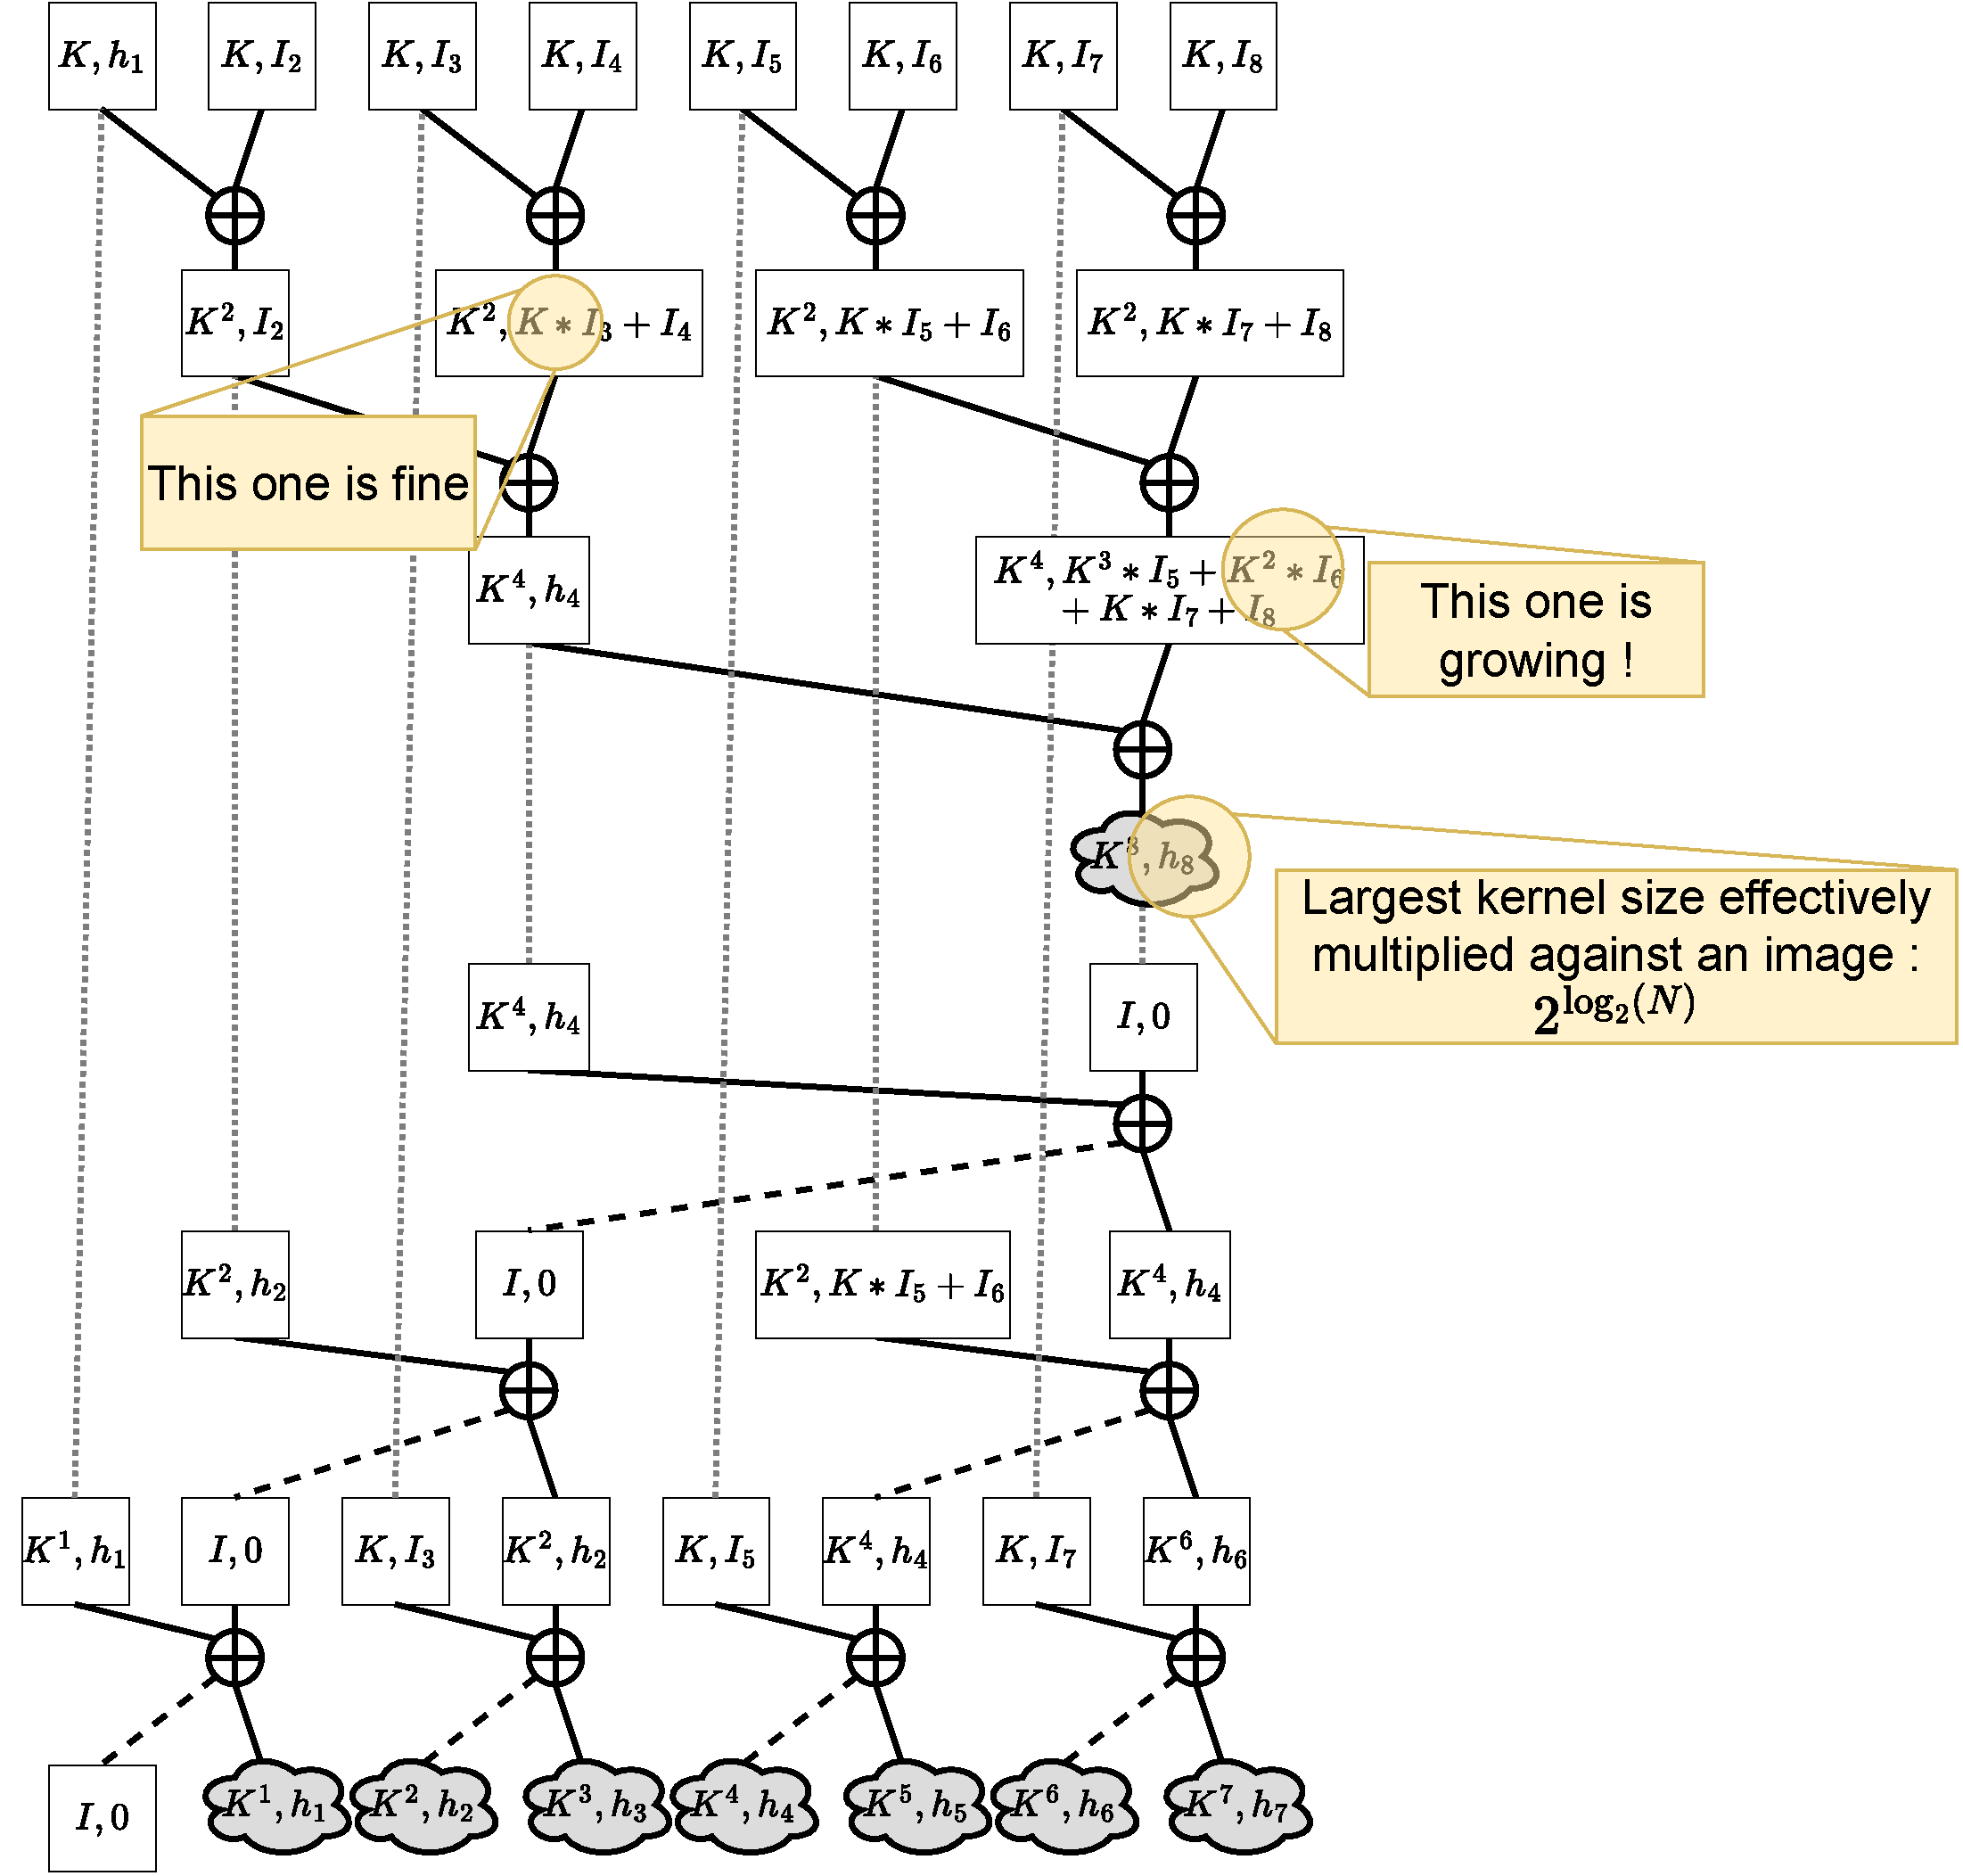
\includegraphics[height=0.3\textheight]{figures/scan_conv.pdf}
    \caption{Parallel scan applied to the monoid structure defined for spatial convolution SSM. Highlighted is the core of the issue : growing kernels lead to a bottleneck where a single operation has $O(T^2)$ complexity.}
    \label{fig:parallel_scan_conv_spatial}
\end{figure}

\subsection{How spectral domain solves the issue}
\label{sec:spectral_ConvSSM}

To dispell the curse of growing kernels we move to the spectral domain. In this domain, our monoid becomes:
\begin{align}
\label{eq:M_SSM_spectral}
    &M^{\mathrm{Conv}_2}\coloneqq \left\{ a = (\hat{K}, \hat{I})\,\middle|\,\exists (K, I)\in M^{\mathrm{Conv}_1},\Bigl\{
\begin{aligned}
    &\hat{K} = \mathrm{FFT}(K_{\mathrm{padded}})\in \C^{h\times w\times c\times c}\\
    &\hat{I} = \mathrm{FFT}(I)\in \C^{h\times w\times c}
\end{aligned}
\Bigr.\right\}\\
\label{eq:+_SSM_spectral}
    &(\hat{K}_a, \hat{I}_a) +^{\mathrm{Conv}_2} (\hat{K}_b,\hat{I}_b)\coloneqq (\hat{K}_b \odot \hat{K}_a, \hat{K}_b \cdot \hat{I}_a + \hat{I}_b)\\
\label{eq:0_SSM_spectral}
    &0\coloneqq(I, 0)
\end{align}
\noindent with $\odot$ the element-wise matrix multiplication and $\cdot$ the element-wise matrix-vector multiplication. With this operator, the kernel grows no more, the cost is again a constant of time and depth, depending only on $h$, $w$ and $c$. We are thus back to a time complexity for the parallel scan of $O(\log T)$.

\begin{proposition}[Spectral ConvSSM Complexity]
\label{prop:spectral_conv_complexity}
    Let $(M, +) \coloneqq (M^{\mathrm{Conv}_2}, +^{\mathrm{Conv}_2})$ be the monoid defined by \Cref{eq:M_SSM_spectral,eq:+_SSM_spectral,eq:0_SSM_spectral}. Let $(a_i)_{i\in I}\in (M^{\mathrm{Conv}_2})^I$.

\begin{align}
    W&= O(T)\\
    T_\infty&= O(\log_2T)
\end{align}
\end{proposition}

\begin{proof}
The proof of \Cref{prop:scan_integer_complexity} applies with the only difference that now, each $+^{\mathrm{Conv}_2}$ operation has complexity $h \times w \times c^3$ for the kernel-kernel multiplication on the left, $h \times w \times c^2$ for the kernel-image multiplication and $h \times w \times c$ for the image addition on the right. This gives :

\begin{align}
\label{eq:W_spectral}
    W&= O(T \times h \times w \times c^3)\\
\label{eq:T_spectral}
    T_\infty&= O(\log_2T \times h \times w \times c^3)
\end{align}
\end{proof}

% \section{Recurrence kernel parameterisation}

% TODO : capability subsection vs complexity subsection vs optimisation subsection

% capability :
% - log domain : multiplicative dynamics in log domain match biological divisive norms. Write it up properly : K*I + I in spatial or spectral is linear, but K*I + I in cepstral becomes K*I * I in spectral - this is the multiplicative dynamic.
% - scale equivariance through wavelets
% - diagoanlisable vs non diagonalisable comment : tradeoff between complexity (cref(sec:TODO below)) and expressivity.
% - anything else ?

% complexity :
% - log domain : This preserves the complexity analysis of section \cref{sec:spectral_ConvSSM}, as you only need to change $+^{\mathrm{Conv}_2}$ such that the right hand side multiplies element wise the images instead of adding them. Then we can operate in log domain.
% - in the fourier space K*K is in $c^3$, and K*I is in $c^2$ (\cref{eq:W_spectral,eq:T_spectral}) : if every frequency bin is diagonalisable, NPLR (normal plus low rank) or something, then this cost can be cut down to $c$ for both. Question : how to actually parameterise spatial domain to have this spectral property ? Would it be easier to parameterise in fourier with constraints such that the spatial domain of the kernel is still k*k ?
% - anything else ?

% optimisation :
% - log domain : It makes BPTT much easier as exponential behaviors mess up gradients but in log domain it is linear
% - orthogonal convolution : this also controls exponential behavior through eigenvalues of 1, but it comes at the cost of expressivity and doesn't have the divisive behavior in log domain. Maybe combine both log domain and orthogonal convolution ? though with log domain you already have what orthogonal brings to the table so maybe it's a bad idea and you just lose expressivity...
% - anything else ?

\subsection{Taking down the constant}
\label{sec:the_constant}

Now that we have solved the main issue of complexity explosion with time, we tackle the problem of the constant. As mentioned in \Cref{prop:SSM_complexity}, as is, the work complexity is $O(T)$ with a constant that is $O(d^3)$ due to matrix multiplications.
\citet{TODO:S4SSM} proposed to reparameterise the recurrence matrix $A$ to be normal plus low rank (NPLR) in order to reduce this constant from $O(d^3)$ to $O(d)$. The complexity gain comes from the change of basis being absorbed outside of the recurrence such that the recurrence can operate on diagonalized matrices. Note that their approach to parallelization through time uses the convolution view of the SSM, not the parallel scan as proposed by \citet{TODO:S5SSM}.
In our case, this $O(c^3)$ is even more prohibitive as it is repeated over each pixel position, with the total constant being $O(k^2c^3 + hwk^2c^2)$ in the spatial domain, and $O(hwc^3)$ in the spectral domain.

In spatial domain, this parameterization translates to having a shared change of basis $V$ for each $K_{x,y}$. This way, $V$ can be factored our ot the kernel such that the resulting kernel follows~: $\forall x,y, \mathcal{K}_{x,y} = \Lambda_{x,y} + P_{x,y} Q_{x,y}^\top$, where
\begin{itemize}
    \item $\Lambda_{x,y}$ are block diagonal with blocks of rank at most $2$ in real domain, and diagonal with eigenvalues of modulus 1 in complex domain. With the complex view, $\mathcal{K}$ is diagonal plus low rank (DPLR).
    \item $P_{x,y}, Q_{x,y} \in \R^{d\times r}$ are low rank matrices, with rank $r$
\end{itemize}
In spectral domain, and after proper zero padding, such a parameterization yields~:

\begin{align*}
    \forall w_1,w_2, \widehat{\mathcal{K}}_{w_1,w_2} &= \sum_{x,y} \alpha_{w_1,w_2}^{x,y} \mathcal{K}_{x,y}\\
    &= \sum_{x,y} \alpha_{w_1,w_2}^{x,y} \left(\Lambda_{x,y} + P_{x,y} Q_{x,y}^\top\right)\\
    &= \sum_{x,y} \alpha_{w_1,w_2}^{x,y} \Lambda_{x,y} + \sum_{x,y} \alpha_{w_1,w_2}^{x,y}P_{x,y} Q_{x,y}^\top\\
\end{align*}

\noindent where $\alpha_{w_1,w_2}^{x,y} = e^{-2\pi i(\frac{w_1x}{h}+\frac{w_2y}{w})}$. There are a couple issues with this~:
\begin{itemize}
    \item The diagonal terms in spatial domain yield diagonal terms in spectral domain. However, these do not have modulus 1, and thus are not stable.
    \item The spectral term coming from the low rank terms is not low rank anymore : it now has rank up to $k^2r$ instead of $r$. This issue can be solved by fixing $P_{x,y}=p,~Q_{x,y}=q$ to be constants. This way, the associated spectral term is low rank.
\end{itemize}
We can circumvent both issues by parameterizing directly in the spectral domain. The tradeoff is that now,
\begin{itemize}
    \item we are bound to a fixed resolution,
    \item the underlying spatial kernel has arbitrary support.
    \item the number of parameters in spectral domain is $hwc(2r+1)$ compared to $k^2c(2r+1)$ in spatial domain.
\end{itemize}
As \citet{TODO:franck} showed that parameterization of CNNs in spectral domain works just fine, we leave the question of finding a parameterization directly in pixel space to future work. Additionally, \citet{TODO} showed that parameterizing the recurrence through a simple normal matrix is as expressive as the NPLR case. We thus take $r=0$ and drop the low rank terms.

% note : mention that \citet{TODO} showed that NPLR parameterisation is no more expressive than normal, in the case of linear SSMs, so in our case we can just remove it.
